\section{Approach}
MDD from social media aims to predict whether a user suffers from certain mental diseases according to his/her social media postings. 
% \KZ{This sounds more like a def of ``online MDD'' or ``MDD by social media''. Was MDD previous defined? If so, cite.}
This section will introduce the proposed framework for MDD, including symptom-based risky post screening and the Psychiatric Experts Model.
%myw not focusing on what you did, but first make clear why you did it. You introduced the framework of two stages but didn't mention why you did it like this. For example, to better disentangle multiple diseases and promote detection efficiency, we first involve symptoms to screen risky posts...

\subsection{Symptom-based Risky Posts Screening}
\label{sec:symp_screen}
%myw maybe start like: Traditional MDD method processes every single post equally overlooking the fact that not every post from a patient reveals useful information for detection. To facilitate... We screen risky posts first, in particular with disease-dependent symptom information...for multidple disease detection. 

% Traditional MDD method processes every single post in the user's posting history equally overlooking the fact that not every post from a patient reveals useful information for detection (e.g. negative emotions, symptom descriptions). 
To facilitate the performance of the MDD model, as well as provide explainable diagnosis basis, we screen risky posts first, in particular with disease-dependent symptom information, and use the selected posts for multiple disease detection. 

Inspired by the clinical diagnosis of psychiatrists, we assume that posts reflecting \textit{symptoms} of mental disorders suggest high risk. Since healthy individuals rarely have symptom-related posts, posts with symptoms could better separate patients from control users. Hence, unlike the prior methods discussed in \S \ref{sec:intro}, we implement a screening method based on the symptom features extracted by a supervised symptom identification model \cite{Zhang2022SymptomIF}.
% To extract symptom features for screening, we apply the model trained by \citet{Zhang2022SymptomIF} for its inclusion of a well-labeled psychiatric symptom database. 
This model can identify 38 symptom classes from 7 mental diseases with a Mental BERT-based encoder \cite{ji2021mentalbert}. It is trained on a large-scale, multi-disease annotated symptom identification dataset \textit{PsySym}, based on the diagnostic criteria from DSM-5 \cite{american2013diagnostic}. 
%It can get high AUC and F1 on the dataset containing all diseases and control posts.
% Its AUC is 98.54 and F1 (with threshold 0.5) is 67.03

The symptom feature of each post is a 38-dimensional vector, where each dimension is the predicted probability of a certain symptom\footnote{These symptoms are carefully extracted from DSM-5, ensuring there is as little overlap as possible between them.}.
We can then estimate the \textit{risky score} of a post with the \textit{max} predicted probability among all diseases. The top $K$ posts with highest risky score among a user's posting history will be selected as his/her risky posts. 
% To obtain a high risky score in \textit{Sum} pooling, a post must have more symptoms with relatively high probability, while in \textit{Max} pooling, only one high enough probability is needed. 
% \MYW{Is there anything novel about the screening process? If not, consider moving it into experiments part and take it as a data preprocessing method, then you experimented two different pooling methods. If you consider using PsySym as a new method to screen risky posts, make it more obvious. "Different from previous risky screening method, we implement.."}

\subsection{Psychiatric Experts Model}
\label{sec:PsyEx_model}

For user-level MDD, Hierarchical Attention Network~\cite{yang2016hierarchical} (HAN) with post and user-level encoder can be applied to better take advantage of the posts' sequential structure. However, the original HAN structure is not appropriate for our multiple mental disease detection task, because it detects all diseases using a single user representation, failing to catch the characteristics of different diseases. 

\begin{figure}[t]
    \centering
    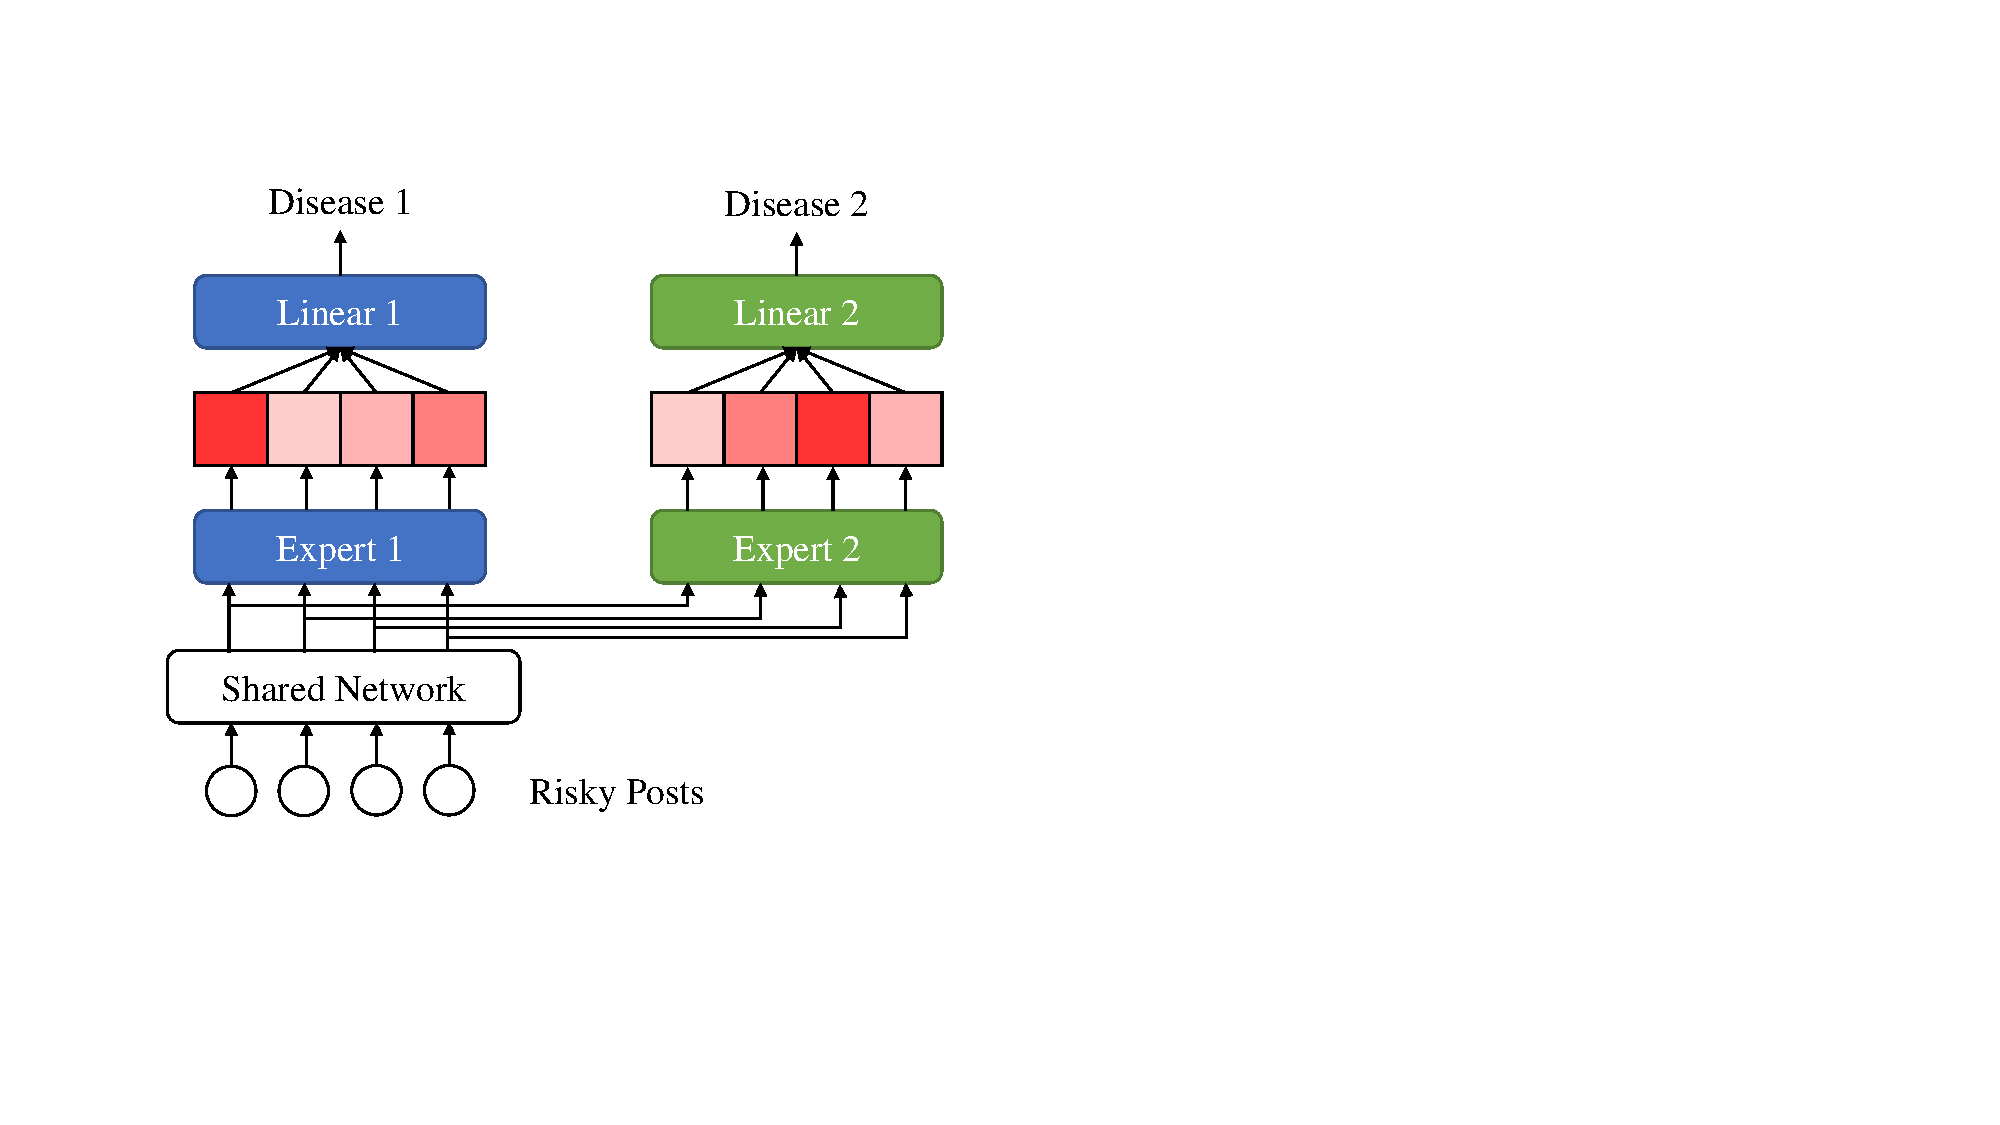
\includegraphics[width=0.8\columnwidth]{figures/model_arch.pdf}
    \caption{Illustration of the proposed model architecture, with 2 disease-specific experts on top of a shared network. Darkness of red
square indicates attention strength, which is different for each disease. }
    \label{fig:model_arch}
\end{figure}

To alleviate this problem, we propose \textit{Psychiatric Experts Model}, which can detect all the mental diseases simultaneously through multi-task learning while still capturing the nuances among them.
It consists of two components: a single shared hierarchical network and $D$ task-specific attention layers on top of the shared backbone, learning the special clues and features like ``experts'' in each disease (See Figure. \ref{fig:model_arch}). 

In the shared part, we employ a pre-trained BERT model as the post encoder and the representation of the [CLS] token as post representation. The user-level encoder utilizes a transformer structure, modeling the relations between these posts $\{p_1, p_2, ..., p_K\}$, and produces updated post representations $\{p'_1, p'_2, ..., p'_K\}$.
% For words $\{w_1, w_2, ..., w_L \}$ in a post, the post representation $p$ is,
% \begin{equation}
%     p = BERT_{[CLS]}(w_1, w_2, ..., w_L)
% \end{equation}
% \begin{equation}
%     p'_1,p'_2, ...,p'_K = Transformer(p_1, p_2, ..., p_K)
% \end{equation}

In the disease-specific part, each disease has its own attention layer to get different attention distributions on the same post sequence. 
As such, these $D$ attention layers can be considered as feature selectors from the shared network \citep{Liu2019EndToEndML}. 
Then we perform a weighted sum of the post representations according to attention score get the distinctive user representations for each disease $d$.
\begin{equation}
    \alpha_{k, d} = \frac{exp(W_d p'_k + b_d)}{\sum_{k'=1}^{K} exp(W_d p'_k + b_d)}
\end{equation}
\begin{equation}
    u_d = \sum_{k=1}^K \alpha_{k, d} p'_k
\end{equation}
where $W_d$ and $b_d$ are both learnable parameters different among diseases. 
Finally, the disease-specific user representation are fed into separate linear layers to get the binary predictions on whether the user suffers from certain mental disease. 

The whole model is trained with the standard binary cross entropy loss, where the loss of all the tasks are averaged. We applied \textit{loss masking} \cite{fonseca2020addressing}, so that
for patients with at least one disease, we do not treat their absent disease labels as negative to alleviate the problem of potentially missing labels. 
%myw "loss caused by users with other diseases"不清楚







